\documentclass[a4paper,oneside,12pt]{article}
\usepackage[utf8]{inputenc}
\usepackage[czech]{babel}
\usepackage{amsmath}
\usepackage{graphicx}

\renewcommand\thefigure{O\arabic{figure}}
\renewcommand\theequation{R\arabic{equation}}


\title{\textbf{Nebojte se složitých rovnic}}
\author{
Michal H. Kolář\footnote{Ústav Maxe Plancka
pro biofyzikální chemii,
Gotinky, Spolková republika Německo}
\and
Vladimír Palivec\footnote{Ústav organické 
chemie a biochemie, Akademie věd České 
republiky, Praha}}
\date{~}

\begin{document}
\maketitle


\begin{quote}
Praktický průvodce fyzikálního chemika
numerickým řešením nelineárních rovnic s jednou
neznámou. (Už rozumíte, proč jsme tohle v nadpisu
opravdu nemohli použít?)
\end{quote}

\begin{center}
\emph{verze 1.0}
\end{center}

\tableofcontents

\newpage

\section{Úvod a motivace}

Fyzikální chemie je vědní obor, který, podobně jako
jiné přírodovědné obory, používá matematický aparát
k zodpovídání otázek na pomezí fyziky a chemie. 
Matematika je vhodný nástroj, nikoli podstata fyzikální
chemie. Jistě by šlo měřit teplotu i bez použití 
matematiky; o tělese pouhým dotykem zjistíme,
zda je teplejší nebo chladnější než jiné těleso. Avšak
se znalostí čísel a operací s nimi se nám otevírá široká 
paleta popisu teploty, se znalostí diferenciálního počtu 
jsme schopni jednoznačně mluvit o teplotních změnách a 
rychlostech těchto změn atp.

Mezi matematikou a přírodními vědami je však jeden zásadní 
rozdíl. Zatímco matematika je věda přesná, v níž musí vše 
do sebe naprosto dokonale zapadat, fyzikální chemie se 
spokojí i s nepřesným řešením. Vždyť i sebelepší měření
neurčí hodnotu fyzikální veličiny zcela přesně.
Uveďme příklad: Hledáme řešení (tzv. kořeny) kvadratické 
rovnice \ref{eq:kvadr}

\begin{equation}
x^2 - 3x - 5 = 0.
\label{eq:kvadr}
\end{equation}
%
Rovnice má dva kořeny: $x_1 = (3 + \sqrt{29}) / 2$
a $x_2 = (3 - \sqrt{29}) / 2$. Jelikož je číslo 29 prvočíslem,
je jeho odmocnina iracionální číslo, tj. má nekonečný 
a neperiodický desetinný rozvoj, anebo jinak, nelze ji 
vyjádřit jako podíl dvou přirozených čísel. Rychlý výpočet
kalkulačkou poskytne $x_1=4,1925824$ a $x_2=-1,1925824$. 
Trochu lepší kalkulačka nebo počítačový program poskytnou
s přesností na 1000 desetinných míst hodnotu (druhý kořen
rovnice si dovolíme vynechat)

\begin{quote}
$x_1$ = \\
4,1925824035 6725201562 5355245770 1647781475 6008082239\\
4418840194 3350083229 8141382934 6438316890 8399177422 \\
0935241089 6972880303 8443107009 9077781347 6608364104 \\
4622643358 6126309260 7340617995 0065262240 0814519435 \\
2263913471 9356847036 9700515844 3597955128 3886298254 \\
1905709747 7920969904 1317448470 8766306701 8208180615 \\
5444371382 7477756182 3970182941 2775911367 2206265037 \\
8958562099 3020629655 1179228059 9027239770 9406563126\\
5536467549 5053443668 5835302906 2337083996 5194270690\\
6187123954 3977273716 0074613440 0568023211 6035505868\\
9307699277 9285510408 5880880190 5197540055 6324181392\\
2214040765 7246107060 5659218170 5381981068 6861441141\\
8969240574 6214576734 6004245653 8995686984 8544548595 \\
4167307029 9897203214 4328698646 2055761488 6119066278 \\
0185895365 6250678663 1816165257 9363933254 9392164950 \\
7210268628 1482849295 8622491960 9219895024 9846636850 \\
4354960334 1536628401 3871220461 5878577098 0356964367 \\
6742668524 0903947640 4786459344 3068341447 5345126833 \\
4702279016 3052849279 9719076037 2204926219 0745700486\\
5127604929 7840840964 8188742048 7031956547 6397620263.\\
\end{quote}
%
Běžně bychom brali tato čísla jako správná řešení výše 
zmíněné kvadratické rovnice, ale buďme na chvíli pedanti
a uvědomme si, že oba výsledky z kalkulačky, ba i z počítače
jsou pouze přibližná (tj. zaokrouhlená) řešení. Na druhou 
stranu, a to je důležité, pokud by $x$ byl např. rozměr
v jednotkách metrů, hodnota 4,1925824 m by byla 
nejspíše dostačující,\footnote{Což neplatí např. u měření
Avogadrovy konstanty, při němž byl určen průměr 
kilogramové křemíkové koule s přesností několika desetin nanometru.}
protože jen málo měřidel umí určit délku tak přesně.

Mnoho rovnic umíme řešit pomocí sady \uv{dovolených}
matematických úprav, případně pomocí vzorců, které si buď
pamatujeme, nebo je máme napsané na taháku. Kvadratická 
rovnice \ref{eq:kvadr2}

\begin{equation}
2x^2 - 6x - 10 = 0
\label{eq:kvadr2}
\end{equation}
%
je jaksi jiná než \ref{eq:kvadr}, avšak má stejné dva 
kořeny. Je nabíledni, že všechny koeficienty rovnice 
\ref{eq:kvadr2} jsou přesně dvojnásobné vůči koeficientům 
v rovnici \ref{eq:kvadr} (\ref{eq:kvadr2} je
dvojnásobkem \ref{eq:kvadr}). 

Není těžké uvěřit, že 
existují rovnice, jejichž kořeny nelze jednoduše vyjá-dřit
tzv. analyticky. Tím máme na mysli, že nelze řešení vyjádřit
formou \uv{$x = \ldots$}.
Příkladem nechť je rovnice \ref{eq:exp}.\footnote{Pravda
to je pouze 
v rozsahu středoškolské matematiky. Zvídavý čtenář může 
dohledat klíčové sousloví Lambertova W-funkce.} 

\begin{equation}
e^x = x^2
\label{eq:exp}
\end{equation}
%
Cílem tohoto textu je osvětlit, proč rovnice, která nemá
(středoškolákovi dostupné) analytické řešení, není bezcenná. 
Text je návodem, jak řešit tímto způsobem komplikované 
rovnice s jednou neznámou. Postupně si v textu ukážeme, jak 
dojít k přibližnému \uv{řešení}. Uvozovky jsou zde na místě,
neboť se nejedná o skutečné řešení rovnice, ale jen o jeho
přibližnou hodnotu. Ta, jak již bylo zmíněno, udělá 
fyzikálnímu chemikovi stejnou radost, jako řešení přesné.


\section{Využití grafů funkcí}

Všimněme si nyní souvislosti mezi funkcemi a rovnicemi.
Funkce jsou matematická přiřazení čísel ze dvou množin; 
\emph{funkce} přiřazuje každému číslu z definičního 
oboru právě jedno číslo z oboru hodnot. Naproti tomu 
\emph{rovnice} dává do souvislosti dvě funkce, jednu
na levé a další na pravé straně od znaménka \uv{=}, 
přičemž nás obvykle zajímá, která čísla z definičních oborů 
obou funkcí poskytují tatáž čísla z oborů hodnot. Číslům,
která požadavku vyhovují, říkáme
kořeny rovnice, neboli řešení rovnice.

Rozveďme příklad rovnice \ref{eq:exp}. Funkci na levé straně
rovnice označíme $f(x) = e^x$ a funkci na pravé straně rovnice
pojmenujme $g(x) = x^2$. Umíme-li sestrojit grafy funkcí
$f(x)$ a $g(x)$, kořen rovnice získáme dohledáním hodnoty
$x$, ve které se oba grafy protínají 
(obrázek \ref{fig:krizeni}). Poznamenejme,
že hodnot může být v závislosti na tvaru rovnice víc, stejně
jako nemusí existovat ani jedna.\footnote{Zkuste sestrojit
grafy $e^x$ a $-x^2$ a dohledat
kořeny rovnice $e^x = -x^2$.}

\begin{figure}
\begin{center}
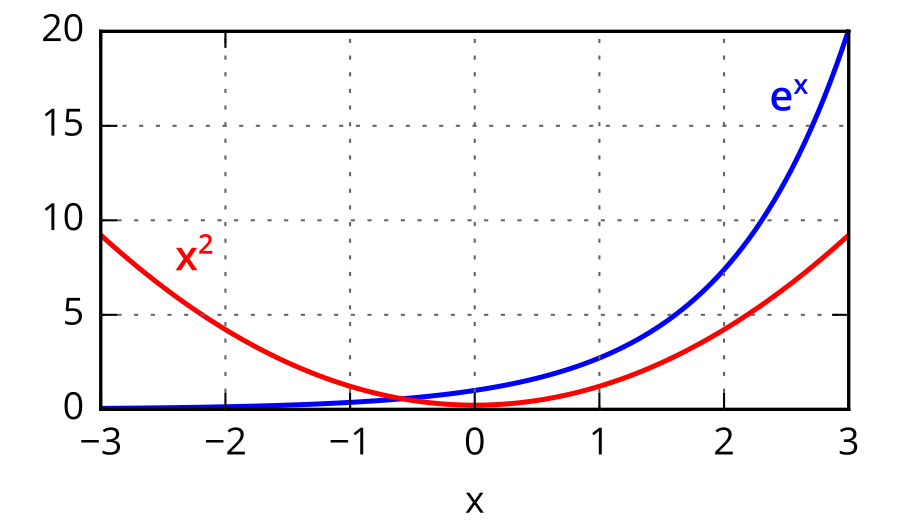
\includegraphics{./IMGS/krizeni-drawing.png}
\end{center}
\caption{Grafy funkcí $e^x$ a $x^2$. Hodnota $x$, ve které
se grafy kříží, je řešením rovnice $e^x=x^2$.}
\label{fig:krizeni}
\end{figure}
%
Sestrojit graf funkce na papíře nemusí být jednoduché, proto
je užitečné vzít si na pomoc počítačový program, tzv. tabulkový
procesor. Nabízí se např. Microsoft Excel, nebo jeho volně
šiřitelná obdoba Libre Office Calc.\footnote{Dostupné 
v češtině zdarma pro několik operační systémů 
na \texttt{https://cs.libreoffice.org}. Jinou alternativou je online
služba \texttt{https://drive.google.com}.} Ten budeme používat i 
v tomto přípravném textu, majíce na paměti značnou podobnost obou 
programových balíků. Proto by ani uživatel začátečník neměl
mít s provedením výpočtů v MS Excel žádné
problémy.\footnote{Na internetu je množství návodů, jak 
s balíkem MS Office pracovat. 
Např. \texttt{http://www.jaknaoffice.cz}.}

Otevřeme si nový dokument. Do sloupce A budeme zapisovat
hodnoty $x$. Sloupce B a C budou obsahovat vzorce pro výpočet 
funkcí $f(x)$ a $g(x)$.

\begin{enumerate}
\item Zapišme hodnoty $x$ v intervalu mezi $-3,0$ a $3,0$ s 
krokem $0,2$ do sloupce A (obrázek \ref{fig:bunky}).
\item Do buňky B1 zapišme vztah pro výpočet $f(x)$ \uv{=exp(A1)}
(bez uvozovek), ve kterém jsme využili funkce exp() 
implementované v balíku Libre Office.
\item Do buňky C1 zapišme vztah pro výpočet $g(x)$ \uv{=A1*A1}.
Připomeňme, že násobení se v takovýchto programech vyjadřuje 
hvězdičkou *.
\item Vypočtěme $f(x)$ pro všechna $x$.
\item Vypočtěme $g(x)$ pro všechna $x$.
\end{enumerate}

\begin{figure}
\begin{center}
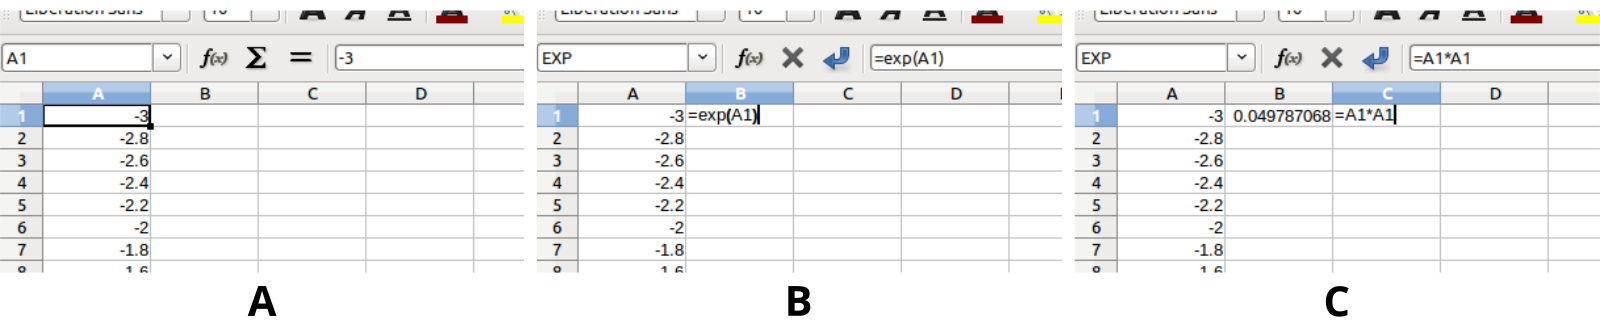
\includegraphics{./IMGS/screens-drawing.png}
\end{center}
\caption{Zadávání hodnot v tabulkovém procesoru Libre Office Calc.}
\label{fig:bunky}
\end{figure}
%
Označíme-li myší všechny hodnoty (včetně hodnot $x$), 
můžeme sestrojit graf pomocí nabídky Vložit/Graf. Objeví
se nové okno, ve kterém vybereme typ grafu \uv{XY (bodový)} a
v pravé části okna vybereme zobrazení s rovnými spojnicemi
(obrázek \ref{fig:grafokno}). Kliknutím na
\uv{Dokončit} přeskočíme další
nastavení a rovnou vytvoříme graf (obrázek \ref{fig:grafy}A).

\begin{figure}
\begin{center}
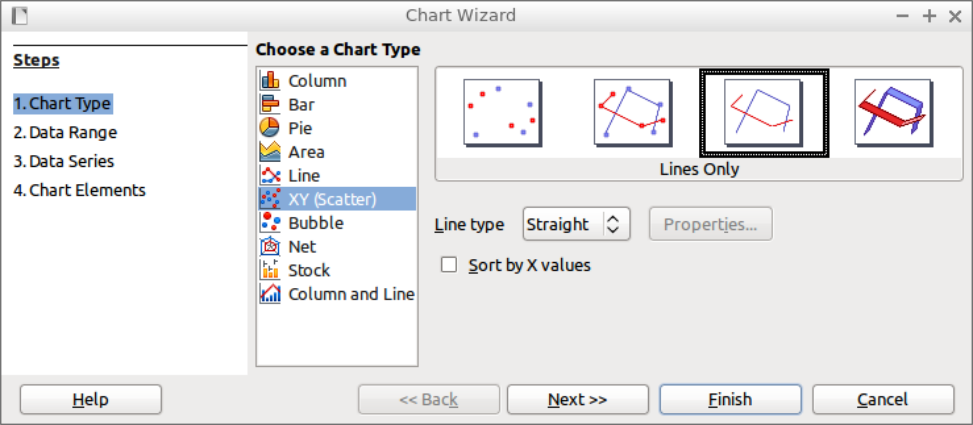
\includegraphics{./IMGS/grafokno-drawing.png}
\end{center}
\caption{Dialogové okno pro tvorbu grafů v tabulkovém procesoru
Libre Office Calc.}
\label{fig:grafokno}
\end{figure}

\begin{figure}
\begin{center}
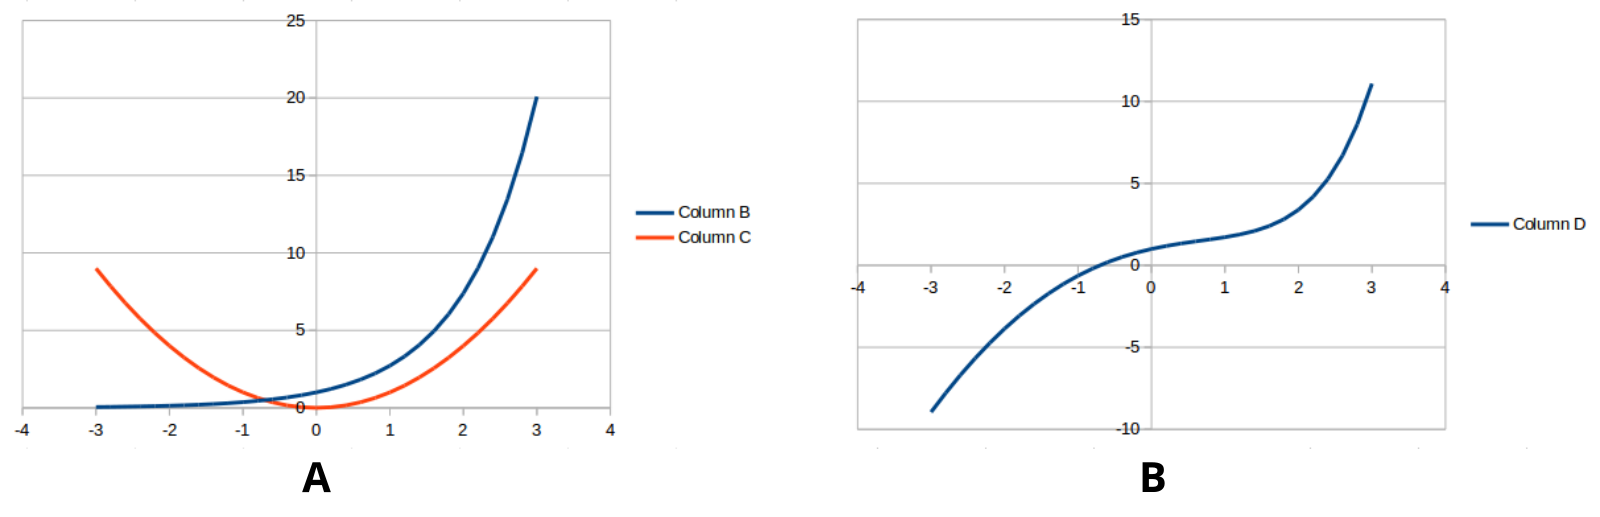
\includegraphics{./IMGS/grafy-drawing.png}
\end{center}
\caption{Grafy vytvořené v tabulkovém editoru Libre Office Calc.}
\label{fig:grafy}
\end{figure}
%
V grafu by měly být dvě křivky -- exponenciála a parabola.
Jejich průsečík, řešení rovnice R3, leží někde mezi $-1$ a $-0,5$,
tedy okolo $-0,75$. Můžeme proto prohlásit, že přibližnou
hodnotou řešení rovnice \ref{eq:exp} je $-0,75$.

S ohledem na následující kapitoly v tomto textu je vhodné
si uvědomit, že každá rovnice se dá vyjádřit ve tvaru,
kde na pravé straně je 0. Rovnice \ref{eq:exp} je
proto ekvivalentní rovnici \ref{eq:exp0}.

\begin{equation}
e^x - x^2 = 0
\label{eq:exp0}
\end{equation}
%
Rovnice dává do souvislosti opět dvě funkce, na každé straně 
od znaménka \uv{=} jednu, přičemž na pravé straně je funkce konstantní 
$m(x) = 0$. V počítačovém dokumentu můžeme snadno vypočítat
hodnoty funkce $n(x) = e^x - x^2$ do sloupce D. Do buňky D1
zapíšeme \uv{=exp(A1) - A1*A1} a výpočet provedeme i pro 
všechna ostatní $x$. Myší označíme hodnoty $x$ a (se stisknutým
Ctrl) i hodnoty ve sloupci D. Graf sestrojíme obdobně jako
v předchozím případě (obrázek \ref{fig:grafy}B). Řešením rovnice \ref{eq:exp0}
(a potažmo i \ref{eq:exp}) je hodnota $x$, ve které graf protíná 
přímku $y=0$.
V tomto bodě je totiž funkční hodnota rovna nule, jak
požaduje rovnice \ref{eq:exp0}.

Stojí za povšimnutí, že odhad řešení \ref{eq:exp0} můžeme získat i bez
vykreslování grafu přímo z tabulky hodnot. Přibližné řešení totiž
bude ležet mezi hodnotami $x$, mezi kterými ve sloupci D dochází
ke změně znaménka. Jinými slovy pomyslný graf v tomto 
intervalu protíná osu $x$. V našem dokumentu tedy řešení
rovnice R4 leží mezi 
$x=-0,8$ a $x=-0,6$. Co takhle vypočítat hodnoty funkce $n(x)$ 
v tomto intervalu, avšak s krokem $0,01$? Poslouží nám třeba 
sloupce G a H. Mezi kterými dvěma $x$ se mění znaménko funkce
$n(x)$? Pokud jste až do této chvíle postupovali jako my, potom
potvrdíte, že řešení \ref{eq:exp0} leží mezi $-0,71$ a $-0,70$.
Postupným \uv{zjemňováním} intervalu lze získat řešení \ref{eq:exp0}
s libovolnou, avšak konečnou, přesností. No není to skvělé?


\section{Metoda půlení intervalů}

Lze tento postup nějak zautomatizovat? A co dělat, když při sobě
nemám počítač, ale jen \uv{hloupou} kalkulačku? Pomůže nám 
tzv. metoda půlení intervalů. Pokusme se ji nyní použít na 
dohledání přibližné hodnoty řešení rovnice, která má na 
pravé straně 0, tedy např. rovnice \ref{eq:exp0}. Na začátku 
potřebujeme dvě čísla, označíme je $x_{1?}$ a $x_{2?}$, 
která leží blízko přesnému řešení. Že se jedná o zkusmé hodnoty
zdůrazňujeme otazníkem. Dále budeme vyžadovat, aby funkční
hodnoty v těchto bodech měly opačná znaménka. Ze zkušenosti
s grafickým zobrazením víme, že řešení leží 
mezi $x_{1?} = -1,0$ a $x_{2?} = -0,5$ (obrázek \ref{fig:grafy}B).

V dalším kroku vypočítáme funkční hodnoty ve zvolených bodech
a taky v bodě $x_{3?}$, který je aritmetickým průměrem oněch bodů.
Fakticky interval $\langle x_{1?}, x_{2?} \rangle$
třetím bodem rozpůlíme. Dostaneme

\begin{align*}
x_{1?} = {} & -1,0  &  n(x_{1?}) = {} & -0,632 \\
x_{2?} = {} & -0,5  &  n(x_{2?}) = {} & 0,357 \\
x_{3?} = {} & -0,75 &  n(x_{3?}) = {} & -0,090. \\
\end{align*}
%
Protože řešení R4 leží v průsečíku grafu $n(x)$ a $m(x)=0$ 
(obrázek \ref{fig:grafy}B), z vypočítaných hodnot 
ve třech zkusmých bodech 
vyplývá, že průsečík leží mezi $-0,75$ a $-0,5$. 
V dalším kroku tedy rozpůlíme tento interval, ve 
kterém funkce $n(x)$ mění znaménko. Dostaneme 
$x_{4?} = -0,625$ a $n(x_{4?}) = 0,145$ a dovodíme, že 
řešení existuje mezi $-0,75$ a $-0,625$. Takto můžeme 
pokračovat, až dosáhneme požadované přesnosti přibližného 
řešení, nebo až nás přestane počítání s kalkulačkou bavit.
Metodu půlení intervalů můžeme chápat taky jako pokus
dostat se půlícím bodem co nejblíž k přesnému řešení rovnice.
A vskutku, každým půlením je funkční hodnota v půlícím bodě blíže
nule, jak ozřejmuje obrázek \ref{fig:puleni}.

\begin{figure}
\begin{center}
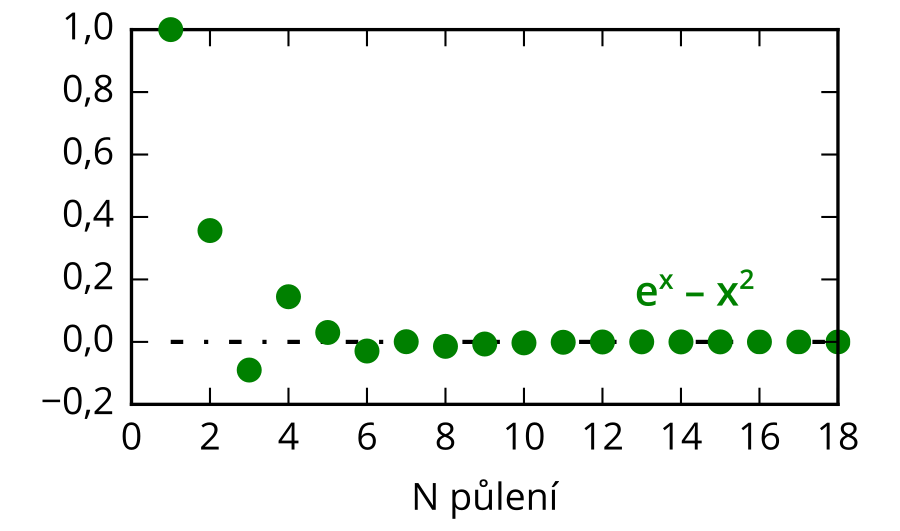
\includegraphics{./IMGS/puleni-drawing.png}
\end{center}
\caption{Hodnota funkce $e^x - x^2$ v závislosti na počtu půlení
intervalů. Správné řešení 0 je vyznačeno čerchovanou čarou.}
\label{fig:puleni}
\end{figure}


\section{Metoda tečen}

Na podobném principu, tedy na hledání průsečíků s přímkou
$y=0$, které se
postupně přibližují přesnému řešení, je založena i metoda tečen.
Ta se někdy nazývá Newtonova nebo Newtonova-Raphsonova metoda.
Rádi bychom upozornili, že metoda tečen představuje maximum, které
řešitel chemické olympiády může upotřebit. Středoškolsky vzdělaného
fyzikálního chemika obvykle nezajímá řešení elegantní, nýbrž 
efektivní ve smyslu vysokého poměru kvality výsledku a
vynaložené úsilí. Z tohoto pohledu je výhodnější držet se tabulkového 
procesoru eventuálně metody půlení intervalů a metodu tečen 
uvádíme jen pro její zajímavost.

K představení metody tečen je potřeba zavést pojem derivace
funkce $f(x)$. My pojem derivace zavedeme velmi hrubě a dovolíme
si odkázat laskavého čtenáře na jiné texty, které se tématu 
derivací věnují obšírněji.\footnote{Jako vhodný začátek může 
sloužit studijní text k Fyzikální olympiádě: Jarešová, 
Volf -- Diferenciální počet ve fyzice, dostupný online 
\texttt{http://fyzikalniolympiada.cz/texty/matematika/difpoc.pdf}.}
Je-li zadaná funkce $f(x)$ 
\uv{slušně vychovaná},\footnote{Formálně musí být funkce $f(x)$
spojitá a mít ve svých bodech vlastní limity. Neformálně musí být
možné graf funkce nakreslit jedním tahem a nesmí obsahovat 
špičky.} můžeme v každém jejím bodě definovat 
její derivaci, která vyjadřuje, jak prudce funkce $f(x)$ roste nebo 
klesá. Nutno zdůraznit, že strmost funkce $f(x)$ je také závislá na
proměnné $x$: pro různá $x$ může být strmost $f(x)$ rozdílná. Derivaci 
funkce $f(x)$ označujeme $f'(x)$. Dá se např. ukázat, že derivace 
funkce v daném bodě je rovna tangens $\alpha$, kde $\alpha$ je úhel,
který svírá tečna v daném bodě s osou $x$. $\mathrm{Tg\,} \alpha$ se též 
nazývá směrnice tečny. Obrázek \ref{fig:tecny} ukazuje tečny ve dvou různých
bodech. Z obrázku je také zřejmé, že derivace v bodě $x_B$ je
větší než v bodě $x_A$: okolo bodu $x_B$ je graf funkce
strmější než v okolí bodu $x_A$.

\begin{figure}
\begin{center}
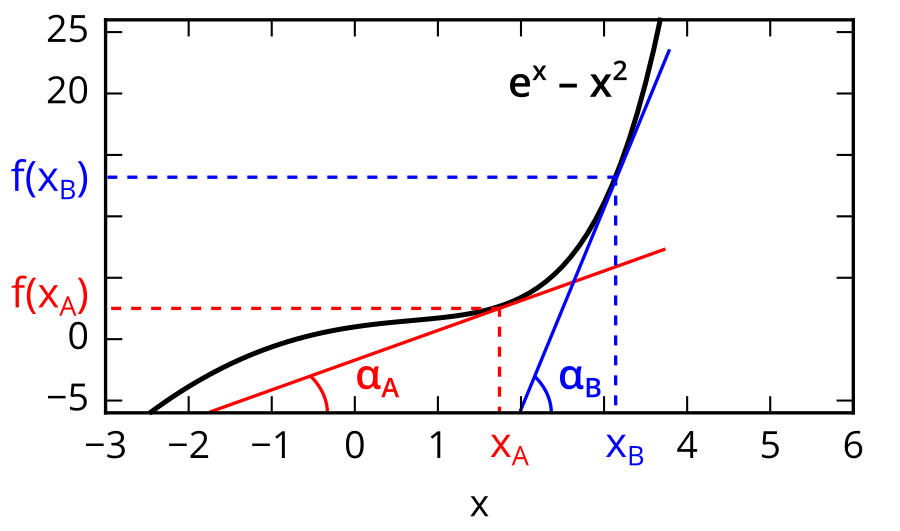
\includegraphics{./IMGS/tecny-drawing.png}
\end{center}
\caption{Závislost úhlu $\alpha$, který svírá tečna s osou $x$,
na bodu, v němž je tečna sestrojena.}
\label{fig:tecny}
\end{figure}
%
Pro derivování a počítání s derivacemi platí několik pravidel,
která bez důkazu uvádíme níže:

\begin{align*}
f(x) = {} & C    & f'(x) = {} & 0, \mathrm{\,kde\,C\,je\,konstanta}  \\
f(x) = {} & x^n    & f'(x) = {} & n x^{n-1} \\
f(x) = {} & \sin x & f'(x) = {} & \cos x \\
f(x) = {} & \cos x & f'(x) = {} & - \sin x \\
f(x) = {} & \ln x  & f'(x) = {} & 1/x \\
f(x) = {} & e^x    & f'(x) = {} & e^x \\
\end{align*}

% alternativní zápis tabulkou je dost ošklivej
% \begin{table}
% \begin{tabular}{ll}
% \hline
% \hline
% $f(x)$ & $f'(x)$ \\
% \hline
% $C     $& $0, \mathrm{\,kde\,C\,je\,konstanta}$ \\
% $x^n   $& $n x^{n-1}$\\
% $\sin x$& $\cos x$\\
% $\cos x$& $- \sin x$\\
% $\ln x $& $1/x$\\
% $e^x   $& $e^x$\\
% \hline
% \hline
% \end{tabular}
% \caption{Vzorce pro výpočty derivací několika běžných funkcí.}
% \end{table}

\begin{align*}
[C \cdot f(x)]' = {} & C \cdot f'(x), \mathrm{\,kde\,C\,je\,konstanta} \\
[f(x) + g(x)]' = {} & f'(x) + g'(x) \\
[f(x) \cdot g(x)]' = {} & f'(x) \cdot g(x) + f(x) \cdot g'(x) \\
\left[ f\left(g(x)\right)\right]' = {} & f'\left(g(x)\right) \cdot g'(x)
\end{align*}
%
Bez souvislosti k fyzikálně-chemickým úlohám si komentář 
zaslouží dvě funkce. Jak známo, $\sin x$ je funkce periodická:
periodicky roste a klesá s periodou $2\pi$, a proto by 
nemělo překvapit, že její derivace je taktéž funkce 
periodická, a to $\cos x$ (obrázek \ref{fig:sincos}).
Všimněte si, že v místech, 
kde $\sin x$ nabývá maxima nebo minima, je strmost $\sin x$
nula (úhel, který svírá tečna v těchto bodech s osou x je 
nulový). Stejně tak je v těchto bodech i 
hodnota $\cos x$ rovna nule. Druhou zajímavou funkcí 
je $e^x$.\footnote{Ta je oproti $\sin x$ z hlediska fyzikální
chemie mnohem důležitější. Funkce $e^x$ se vyskytuje 
např. v rovnicích
radioaktivních rozpadů, nebo obecněji v popisu chemických
reakcí 1. řádu.} Derivováním $e^x$ dostaneme opět $e^x$, což 
znamená, že funkční hodnota v bodě $x$ je přímo rovna
směrnici tečny v daném bodě.

\begin{figure}
\begin{center}
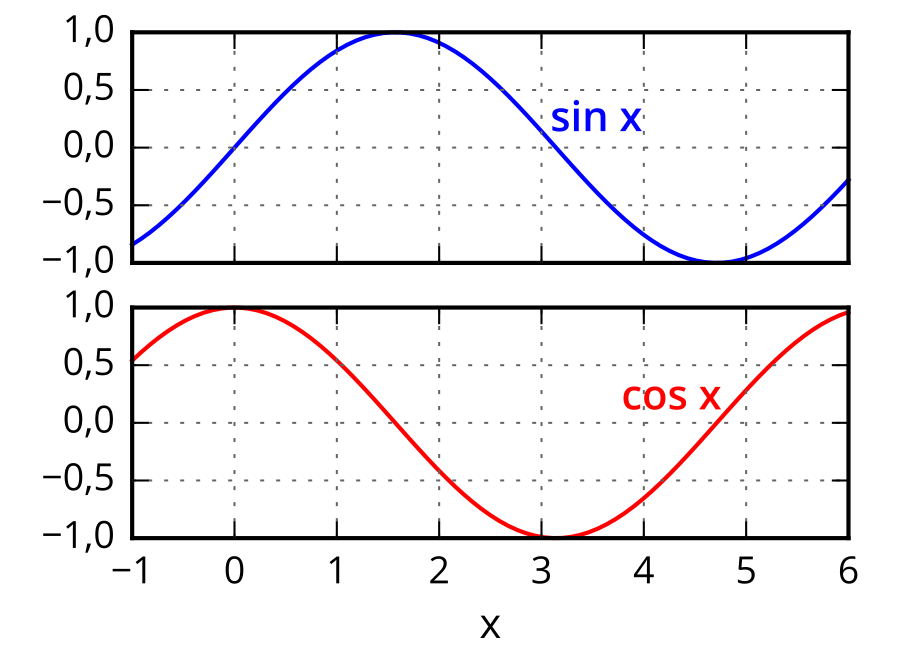
\includegraphics{./IMGS/sincos-drawing.png}
\end{center}
\caption{Funkce sinus (sin x) a kosinus (cos x).}
\label{fig:sincos}
\end{figure}
%
Ale zpět k řešení rovnice \ref{eq:exp0}. Pro odhad 
přibližné hodnoty řešení zvolíme zkusmý bod
$x_{1?}=1,5$.\footnote{Zkusmý bod by měl být dostatečně 
blízko přesnému řešení. My z důvodu názornosti volíme 
trochu vzdálenější bod než v metodě půlení intervalů.}
V tomto bodě spočítáme funkční hodnotu $f(x_{1?})$ a její
derivaci $f'(x_{1?})$. Tečna protíná přímku $y=0$ v bodě $x_{2?}$
a vytváří pravoúhlý trojúhelník (obrázek \ref{fig:trojuh}).
Pro bod $x_{2?}$ platí

\begin{equation*}
\mathrm{tg\,} \alpha = \frac{f(x_{1?})}{x_{1?} - x_{2?}}.
\end{equation*}
%
Ze vztahu mezi derivací a úhlem tečny potom

\begin{equation*}
\mathrm{tg\,} \alpha = f'(x_{1?}),
\end{equation*}
%
a tedy

\begin{equation*}
x_{2?} = x_{1?} - \frac{f(x_{1?}) }{f'(x_{1?})}.
\end{equation*}
%
Zbývá vypočítat hodnotu derivace v bodě $x_{1?}$. Nejdříve
zderivujeme funkci $n(x) = e^x - x^2$, kde využijeme 
pravidla shrnutá výše.

\begin{align*}
n'(x) = {} & (e^x - x^2)' = \\
	  = {} & (e^x)' + (-1 \cdot x^2)' = \\
      = {} & e^x - 1 \cdot (x^2)' = \\
      = {} & e^x - 2x
\end{align*}
%
Dosazením $x_{1?}=1,5$ dostaneme $x_{2?}=-0,006$. 

\begin{equation*}
x_{2?} = 1,5 - \frac{e^{1,5} - 1,5^2}{e^{1,5} - 2 \cdot 1,5} = -0,006
\end{equation*}
%
Bod $x_{2?}$ se nachází blíž přesnému řešení 
rovnice \ref{eq:exp0}, které je na obrázku \ref{fig:trojuh} 
zachyceno průsečíkem grafu funkce a funkce $m(x)=0$.

\begin{figure}
\begin{center}
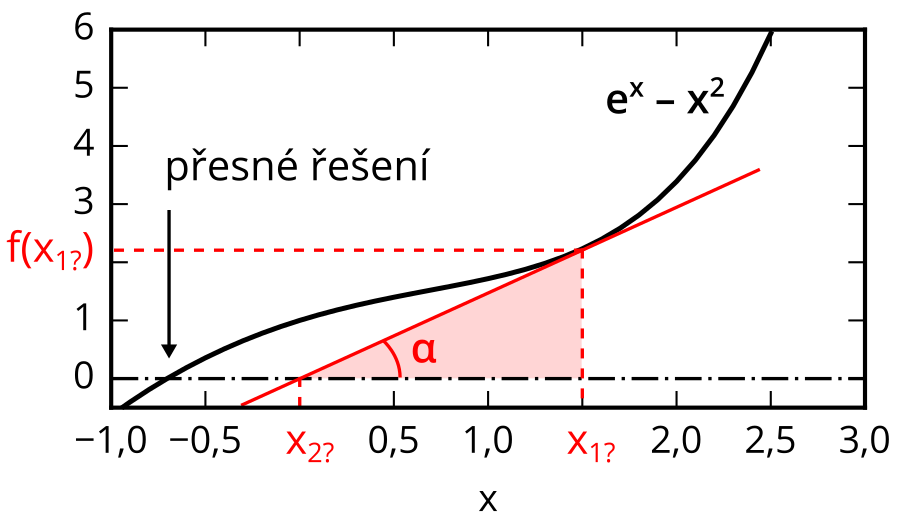
\includegraphics{./IMGS/trojuh-drawing.png}
\end{center}
\caption{První krok v metodě tečen. První zkusmý bod $x_{1?}$,
v něm sestrojená tečna k funkci $e^x - x^2$ (červeně)
a její průsečík s přímkou $y=0$
(čerchovaně) definují trojúhelník (růžově) 
využitý k výpočtu bodu $x_{2?}$.}
\label{fig:trojuh}
\end{figure}
%
V dalším kroku sestrojíme tečnu v bodě $x_{2?}$, dohledáme
její průsečík s osou x, který použijeme v dalším kroku metody.
Tímto způsobem můžeme pokračovat až do chvíle, kdy se dva 
následující průsečíky s přímkou $y=0$,
nebo funkční hodnoty v těchto bodech, liší 
o méně než předem vybraný práh. Ve srovnání s metodou 
půlení intervalů dosáhneme obvykle výsledku pomocí menšího počtu kroků.
V případě rovnice \ref{eq:exp0} a zvolené přesnosti na 4 desetinná
místa tedy v 6 krocích metodou tečen a v 18 krocích metodou 
půlení intervalů.


\section{Aplikace ve fyzikální chemii}

Uvedeme jeden příklad, jak numerické metody použít k řešení
fyzikálně-chemických problémů. Začneme stavovou rovnicí plynu.
Dle J. D.  van der Waalse\footnote{nizozemský fyzik (1837--1923),
nositel Nobelovy ceny za fyziku (1910)}
platí pro tlak $p$ a molární 
objem $V_m$ reálného plynu následující vztah, tzv. van der Waalsova
(vdW) stavová rovnice.

\begin{equation}
p = \frac{RT}{V_m - b} - \frac{a}{V_m^2},
\label{eq:vdw}
\end{equation}
%
kde $R$ je univerzální plynová konstanta, $T$ termodynamická teplota,
a $a$ a $b$ jsou parametry rovnice, které se vztahují ke studovanému
plynu.

Otázka může znít, jaký je molární objem oxidu uhličitého při teplotě
$T=373$\,K a tlaku $p=5,07$\,MPa. Parametry pro oxid uhličitý jsou
následující $a = 0,365$ J\,m$^3$\,mol$^{-2}$,
$b = 4,28 \cdot 10^{-5}$ m$^3$\,mol$^{-1}$. 
Rovnici \ref{eq:vdw} lze upravit do tvaru

\begin{equation}
V_m^3 - \left ( \frac{RT}{p} + b \right ) V_m^2 +
\frac{a}{p} V_m - \frac{ab}{p} = 0. 
\label{eq:vm}
\end{equation}
%
Z rovnice \ref{eq:vm} je patrné, že se jedná o rovnici kubickou vzhledem
k molárnímu objemu $V_m$. Ačkoli existují způsoby, jak si s kubickou rovnicí
poradit analyticky,\footnote{Viz Cardanovy vzorce.} my zkusíme vypočítat
její kořeny numericky pomocí metody půlení intervalů. 
Kubická rovnice může mít nula až tři reálné kořeny, proto je
důležité mít rozumný odhad prvních dvou zkusmých bodů. K tomu nám poslouží
molární objem vypočítaný pomocí stavové rovnice ideálního plynu:

\begin{equation}
p = \frac{RT}{V_{m,id}}
\label{eq:ig}
\end{equation}
%
Dosazením dostaneme přibližně $V_{m,id} = 6,11 \cdot 10^{-4}$\,m$^3$,
z čehož odhadneme, že by řešení vdW rovnice \ref{eq:vm} mohlo existovat
v intervalu mezi $V_{m,1?} = 10^{-3}$\,m$^3$ a $V_{m,2?} = 10^{-4}$\,m$^3$.
Vypočteme hodnoty pro krajní body počátečního intervalu a také pro půlící
bod. Levou stranu rovnice \ref{eq:vm} označíme LS.

\begin{align*}
V_{m,1?} = {} & 10^{-3} \mathrm{\,m^3}  &  LS(V_{m,1?}) = {} & 4,14450 \cdot 10^{-10} \\ 
V_{m,2?} = {} & 10^{-4} \mathrm{\,m^3}  &  LS(V_{m,2?}) = {} & -1,4266 \cdot 10^{-12} \\ 
V_{m,3?} = {} & 5,5 \cdot 10^{-4} \mathrm{\,m^3}  &  LS(V_{m,3?}) = {} & 4,91490 \cdot 10^{-12} \\ 
\end{align*}
%
Neměla by nás znepokojit velmi malá čísla levé strany rovnice, která
pro nezkušené oko mohou být dostatečně blízko požadované nule. Musíme
si však uvědomit, že rozdíly molárních objemů jsou v řádech $10^{-4}$ m$^3$,
neboli ve stovkách ml, což je patrně přesnost nedostačující.

Dovodíme, že řešení leží mezi $V_{m,2?}$ a $V_{m,3?}$, z nichž následně
vypočteme aritmetický průměr $V_{m,4?}$ a levou stranu rovnice.

\begin{align*}
V_{m,4?} = {} & 3,25 \cdot 10^{-4} \mathrm{\,m^3}  &  LS(V_{m,4?}) = {} & -1,44832 \cdot 10^{-11} \\ 
\end{align*}
%
Po deseti opakováních dojdeme k výsledku $V_m$ = 529 ml. Tato hodnota
se od ideálního chování odchyluje přibližně o 13\%. To můžeme považovat za
významnou odchylku a prohlásit, že oxidu uhličitý se za daných podmínek
nechová ideálně. Připomeňme, že reálné plyny mají blízko ideálnímu chování
pouze za vysokých teplot a nízkých tlaků.


\section{Závěrečné poznámky}

Mohlo by se zdát, že numerický přístup k rovnicím pomocí metody tečen
nebo půlení intervalů přemůže všechny nesnáze s jejich řešením.
Není tomu bohužel tak. S komplikovaností rovnic rostou i nároky 
na počáteční odhady řešení a špatná volba může snadno vést k neúspěchu.
Neúspěch si můžeme představit např. jako situaci, kdy se nové body
nepřibližují skutečnému řešení, nebo se k němu přibližují jen velmi pomalu.
Říkáme, že metoda špatně konverguje (obrázek \ref{fig:konverg}).
Jiným druhem problémů je konvergence k jinému řešení, než je 
požadováno/předpokládáno.

Doplňme ještě, že na internetu je dostupná řada aplikací, které
poskytují numerická řešení. Často implementují některou z předkládaných
metod. Za povšimnutí stojí především (z našeho pohledu velmi mocná) 
služba na \texttt{http://www.wolframalpha.com}, se kterou vám stejně
jako s úlohami Chemické olympiády přejeme spoustu zábavy.

\begin{figure}
\begin{center}
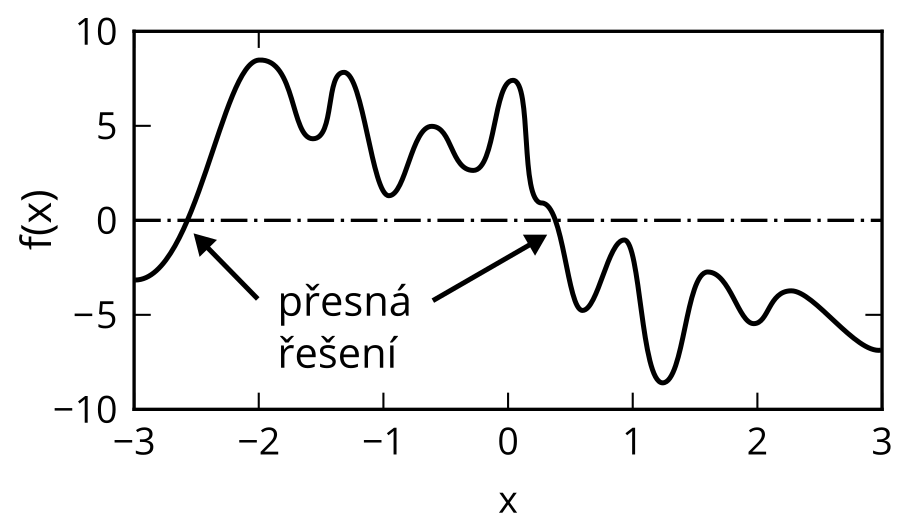
\includegraphics{./IMGS/konverg-drawing.png}
\end{center}
\caption{Funkce $f(x)$, jejíž rovnici $f(x) = 0$ bude kvůli špatné
konvergenci obtížné numericky řešit metodou tečen nebo půlení intervalů.}
\label{fig:konverg}
\end{figure}

\section*{Poděkování}

Zde si dovolíme poděkovat vybraným účastníkům Letního odborného
soustře-dění v Běstvině, kteří si po kultovní noční hře Labyrint
místo spánku raději vyslechli přednášku o numerických řešeních
rovnic a svým nadšením a dotazy pomohli zformovat tento text. 
Významné díky patří též Petru Slavíčkovi za pečlivé přečtení 
nulté verze textu.

\section*{Errata}

\end{document}
